\documentclass[12pt,onecolumn,a4paper,fleqn]{article}
\usepackage{epsfig,graphicx,subfigure,amsthm,amsmath}
\usepackage{fancyhdr}
\usepackage{setspace}
\usepackage{sidecap}
\usepackage{tikz}
\usepackage{pgfplots}
\usetikzlibrary{decorations.pathreplacing}
\usepackage{relsize}
\usepackage{color}
\usepackage{files/persianheader}     
\usepackage{float}
\usepackage{enumerate}
\usepackage{booktabs}
\usepackage{xepersian}


\settextfont[Path=fonts/,BoldFont={ZarBd.ttf},BoldFeatures={Scale=0.9}]{BZar.ttf}
\setdigitfont[Path=fonts/,BoldFont={ZarBd.ttf},BoldFeatures={Scale=0.9}]{BZar.ttf}

\pagestyle{fancy}
\fancyhf{}
\rhead{\textbf{علوم اعصاب محاسباتی}}
\chead{\textbf{پروژه‌ی پایانی درس}}
\lhead{\textbf{\nouppercase{\rightmark}}}
\cfoot{({\thepage})}
\renewcommand{\headrulewidth}{1pt}
\renewcommand{\footrulewidth}{1pt}
\renewcommand{\sectionmark}[1]{\markright{#1}}
\renewcommand{\subsectionmark}[1]{\markright{#1}}

\onehalfspacing
\begin{document}
	\relscale{1}
	\neurotitlepage

\section{مقدمه}

توضیحات کلی در مورد کدها و پروژه و مقاله.

\pagebreak

\section{آشنایی با مقاله‌ی پژوهش}

\subsection{هدف پژوهش}
هدف این مقاله مدل سازی \lr{receptive field} نورون‌های پیچیده‌ غشر بصری\footnote{\lr{Visual cortex}} می‌باشد. در واقع با اعمال تحریک‌های تصادفی \lr{spatiotemporal} از توزیع 
$p(s)$
و مشاهده‌ی پاسخ نورون‌ها می‌خواهیم راستایی را بدست بیاوریم که در آن $p(s|r)$ تفاوت معناداری با توزیع اولیه‌ی تحریک‌ها داشته باشد.

تفاوت این مقاله با پژوهش‌های قبل خود آن است که به دلیل رفتار غیر-خطی نورون‌های پیچیده‌ی موجود در \lr{Visual cortex}  نمی‌توانیم از آنالیز‌های خطی 
\lr{spike-triggered average}
که پیش از این کارگشا بودند استفاده کنیم. این مقاله روش 
\lr{spike-triggered correlation analyses}
 را پیشنهاد می‌دهد که بر پایه‌ی \lr{Wiener Kernel} طراحی شده است.

نهایتا با این پژوهش با بررسی‌هایی که انجام می‌دهد ادعا می‌کند که می توان  با این روش پایه‌ای برای تحریک‌ها ارائه داد که تعداد کمی از آن‌ها مشخص کننده‌ی ویژگی‌های مرتبط و تعداد زیادی مربوط به ویژگی‌های پوچ می‌باشند.
\subsection{نورون‌های‌ «پیچیده»}
این مفهوم اولین بار در مقاله‌ی نوبلیست \lr{Hubel and Wiesel} مطرح شده است. نورون‌های ساده نورون‌هایی هستند که رابطه‌ی تحریک-پاسخ آنها نسبت به زمان خطی می‌باشد. این موضوع باعث به وجود آمدن مناطق \lr{ON-OFF} در \lr{Receptive Field} نورون مورد نظر می‌شود. به عکس دست نوشته‌ی موجود در مقاله‌ی مذکور برای جزئیات بیشتر توجه کنید.

\begin{figure}[h]
	\centering
	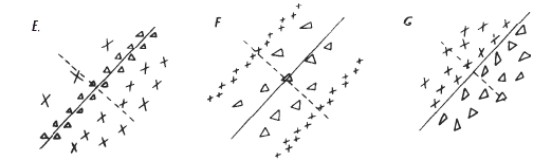
\includegraphics[width=0.8\linewidth]{photos/simple_cells.png}
  \caption[]{مناطق \lr{ON-OFF} حوزه‌ی دریافتی نورون‌های ساده\footnotemark}
\end{figure}
\footnotetext{\lr{EVOLUTION OF IDEAS ON THE PRIMARY
		VISUAL CORTEX, 1955-1978. BY DAVID H. HUBEL}}

همچنین در بخش 
\lr{Material and Methods}
آمده است که اگر نسبت هارمونیک اول به مقدار \lr{DC} حوزه‌ی دریافتی بزرگتر از یک باشد نورون را ساده می‌نامیم. روشن است که نورون‌هایی که از تعاریف بالا پیروی نکنند ساده نبوده و پیچیده‌اند.

\subsection{\lr{STC analysis}}
می‌دانیم که اگر یک ویژگی در تحریک باعث تغییر احتمال اسپایک زدن شود، می‌دانیم که اگه تحریک‌ها را به فضای آن \lr{spike-triggered} منتقل کنیم باید تفاوت قابل توجهی بین مقادیر $p(s|r)$ و $p(s)$ باشد.\footnote{$p(\text{stimulus\ |\ response})$} 

روش‌های مبتنی بر \lr{correlation} با هدف بررسی تغییر این توزیع احتمالات با توجه به تغییرات گشتاور مرتبه‌ی دوم آنها(واریانس) طراحی می‌شوند.

در این بین روش \lr{PCA} به این خاطر که پایه‌ای در اختیار ما قرار می‌دهد که راستا‌های بیشترین تا کمترین واریانس می‌باشند، بسیار مناسب کار ما خواهد بود و می‌تواند ویژگی‌هایی را که در آن واریانس تحریک‌ها بسیار بالا می‌باشد را در اختیار ما بگذارد.

روش \lr{spike-triggered analysis} مبتنی بر موارد فوق مراحل زیر را انجام می‌دهد:
\begin{enumerate}
	\item ابتدا با فرض اینکه حافظه‌ی نورون‌ها بیشتر از ۱۶ فریم یا ۲۶۸ میلی‌ثانیه نخواهد بود؛ پترن‌های تحریک را متشکل از ۱۶ نوار رنگی در ۱۶ فریم و در فضای ۲۵۶ بعدی تعریف می‌کنیم.	
	\item ماتریس \lr{spike-triggered correlation} 
	را به صورت زیر تعریف می‌کنیم:
	$$ C = \frac1N \sum_{i = 1}^{N} S(i)^TS(i) $$
	که در آن $S(i)$ بردار ۲۵۶ بعدی در $i$امین باریست که نورون در طول آزمایش اسپایک زده است و $N$ تعداد کل اسپایک‌ها در طول آزمایش است.
	\item بردارویژه‌ها و مقدارویژه‌های این ماتریس محاسبه شده و با توجه به اندازه‌ی مقدار‌ویژ‌ه‌ها رتبه‌بندی می‌شوند.‌	
\end{enumerate}

با توجه به \lr{PCA} می‌دانیم که حاصل راستا‌هایی خواهد بود که در آن واریانس تحریک‌هایی که موجب اسپایک می‌شوند از زیاد به کم مرتب شده اند.
	
\subsection{اعتبارسنجی نتایج}
برای اعتبارسنجی مشاهدات روش \lr{spike-triggered correlation} روشی که مقاله‌ استفاده می‌کند این است که دنباله‌ای از اسپایک‌های تصادفی با تعداد اسپایک‌های مساوی با $N$ تولید می‌کند و ماتریس \lr{correlation} تحریک‌هایی که موجب این اسپایک‌های فرضی تصادفی شدند را ایجاد می‌کنیم. هدف این است که \lr{control correlation matrix} را محاسبه کنیم که به این معناست که روشی که در قبل پیش گرفتیم را برای داده‌هایی که می‌دانیم مستقل از اسپایک زدن هستند(تمام داده‌ها)نیز اعمال کنیم. با توجه به حجم بالای داده‌ها $N$ مساوی تعداد اسپایک‌ها را در نظر می‌گیریم و ۵ بار فرایند تولید \lr{control correlation matrix} را انجام می‌دهیم و میانگین مقدارویژه‌ها را محاسبه می‌کنیم.با توجه به متن مقاله حاصل این میانگین‌گیری 
$\pm 5.2 SD$ 
بازه‌ی اطمینان ما با $p< 10^{-4}$ خواهد بود. و بنابراین اگر مقدارویژه‌ای خارج از این بازه‌ی اطمینان باشد؛ آن مقدارویژه و بردارویژه دارای تفاوت آشکار خواهند بود.(در واقع آن بردار ویژه راستاییست که تحریک‌های موجب اسپایک در آن واریانس و در نتیجه‌ توزیع احتمال کاملا متفاوتی با توزیع اولیه دارند)
\subsection{نتایج پژوهش}
همانطور که در بخش‌های قبل اشاره کردیم هدف پیدا کردن \lr{eigenvalue}هایی بود که خارج از بازه‌ی اطمینان باشند که آن‌ها به عنوان ویژگی‌های اصلی موجود در \lr{receptive-field} گزارش شود.نتایج مقاله نشان می‌دهد که برای تعداد زیادی از سلول‌های پیچیده دو بردارویژه پیدا شده‌است که این بردار ویژه‌ها ناحیه‌ی \lr{ON-OFF}  مشخص و مجزا ازهمی دارند و همچنین \lr{correlation} بسیار پایینی دارند.همچنین می‌بینیم که این راستا‌ها به خوبی سبب تحریک نورون‌ها می‌شوند با این حال برای \lr{eigenvalue}هایی که در بازه‌ی اطمینان مذکور قرار دارند تاثیر بسیار کمتری در تحریک نورون‌ها مشاهده شده است.
	
\end{document}